\documentclass[11pt,compress,t,notes=noshow, xcolor=table]{beamer}
\usepackage[]{graphicx}\usepackage[]{color}
% maxwidth is the original width if it is less than linewidth
% otherwise use linewidth (to make sure the graphics do not exceed the margin)
\makeatletter
\def\maxwidth{ %
  \ifdim\Gin@nat@width>\linewidth
    \linewidth
  \else
    \Gin@nat@width
  \fi
}
\makeatother

\newcommand{\citebutton}[2]{%
\beamergotobutton{\href{#2}{#1}}%
}

\newcommand{\blu}[1]{\textcolor{blue}{#1}}
\newcommand{\org}[1]{\textcolor{orange}{#1}}
\newcommand{\ques}{\textbf{\textcolor{red}{Question:  }}}
\newcommand{\questionssofar}{\begin{frame}\frametitle{Any questions?}\end{frame}}

\newcommand\warning{%
 \makebox[1.4em][c]{%
 \makebox[0pt][c]{\raisebox{.1em}{\scriptsize!}}%
 \makebox[0pt][c]{\color{red}\normalsize$\bigtriangleup$}}}%

\definecolor{fgcolor}{rgb}{0.345, 0.345, 0.345}
\newcommand{\hlnum}[1]{\textcolor[rgb]{0.686,0.059,0.569}{#1}}%
\newcommand{\hlstr}[1]{\textcolor[rgb]{0.192,0.494,0.8}{#1}}%
\newcommand{\hlcom}[1]{\textcolor[rgb]{0.678,0.584,0.686}{\textit{#1}}}%
\newcommand{\hlopt}[1]{\textcolor[rgb]{0,0,0}{#1}}%
\newcommand{\hlstd}[1]{\textcolor[rgb]{0.345,0.345,0.345}{#1}}%
\newcommand{\hlkwa}[1]{\textcolor[rgb]{0.161,0.373,0.58}{\textbf{#1}}}%
\newcommand{\hlkwb}[1]{\textcolor[rgb]{0.69,0.353,0.396}{#1}}%
\newcommand{\hlkwc}[1]{\textcolor[rgb]{0.333,0.667,0.333}{#1}}%
\newcommand{\hlkwd}[1]{\textcolor[rgb]{0.737,0.353,0.396}{\textbf{#1}}}%
\let\hlipl\hlkwb

\usepackage{framed}
\makeatletter
\newenvironment{kframe}{%
 \def\at@end@of@kframe{}%
 \ifinner\ifhmode%
  \def\at@end@of@kframe{\end{minipage}}%
  \begin{minipage}{\columnwidth}%
 \fi\fi%
 \def\FrameCommand##1{\hskip\@totalleftmargin \hskip-\fboxsep
 \colorbox{shadecolor}{##1}\hskip-\fboxsep
     % There is no \\@totalrightmargin, so:
     \hskip-\linewidth \hskip-\@totalleftmargin \hskip\columnwidth}%
 \MakeFramed {\advance\hsize-\width
   \@totalleftmargin\z@ \linewidth\hsize
   \@setminipage}}%
 {\par\unskip\endMakeFramed%
 \at@end@of@kframe}
\makeatother

\definecolor{shadecolor}{rgb}{.97, .97, .97}
\definecolor{messagecolor}{rgb}{0, 0, 0}
\definecolor{warningcolor}{rgb}{1, 0, 1}
\definecolor{errorcolor}{rgb}{1, 0, 0}
\newenvironment{knitrout}{}{} % an empty environment to be redefined in TeX

\usepackage{alltt}
\newcommand{\SweaveOpts}[1]{}  % do not interfere with LaTeX
\newcommand{\SweaveInput}[1]{} % because they are not real TeX commands
\newcommand{\Sexpr}[1]{}       % will only be parsed by R
\newcommand{\xmark}{\ding{55}}%


\usepackage[english]{babel}
\usepackage[utf8]{inputenc}

\usepackage{dsfont}
\usepackage{verbatim}
\usepackage{amsmath}
\usepackage{amsfonts}
\usepackage{amssymb}
\usepackage{bm}
\usepackage{csquotes}
\usepackage{multirow}
\usepackage{longtable}
\usepackage{booktabs}
\usepackage{enumerate}
\usepackage[absolute,overlay]{textpos}
\usepackage{psfrag}
\usepackage{algorithm}
\usepackage{algpseudocode}
\usepackage{eqnarray}
\usepackage{arydshln}
\usepackage{tabularx}
\usepackage{placeins}
\usepackage{tikz}
\usepackage{setspace}
\usepackage{colortbl}
\usepackage{mathtools}
\usepackage{wrapfig}
\usepackage{bm}
\usepackage{amsmath}
\usepackage{pifont}

\usetikzlibrary{shapes.multipart,shapes,arrows,automata,positioning,calc,chains,trees, shadows}
\tikzset{
  %Define standard arrow tip
  >=stealth',
  %Define style for boxes
  punkt/.style={
    rectangle,
    rounded corners,
    draw=black, very thick,
    text width=6.5em,
    minimum height=2em,
    text centered},
  % Define arrow style
  pil/.style={
    ->,
    thick,
    shorten <=2pt,
    shorten >=2pt,}
}

\tikzstyle{vec}=[draw, rectangle, fill = white, minimum width=5mm, minimum height=1cm, inner sep = 2pt]

\usepackage{subfig}

% Defines macros and environments
\usepackage{../../style/lmu-lecture}


\let\code=\texttt
\let\proglang=\textsf

\setkeys{Gin}{width=0.9\textwidth}

\setbeamertemplate{frametitle}{\expandafter\uppercase\expandafter\insertframetitle}

\usepackage{bbm}
% basic latex stuff
\newcommand{\pkg}[1]{{\fontseries{b}\selectfont #1}} %fontstyle for R packages
\newcommand{\lz}{\vspace{0.5cm}} %vertical space
\newcommand{\dlz}{\vspace{1cm}} %double vertical space
\newcommand{\oneliner}[1] % Oneliner for important statements
{\begin{block}{}\begin{center}\begin{Large}#1\end{Large}\end{center}\end{block}}


%new environments
\newenvironment{vbframe}  %frame with breaks and verbatim
{
 \begin{frame}[containsverbatim,allowframebreaks]
}
{
\end{frame}
}

\newenvironment{vframe}  %frame with verbatim without breaks (to avoid numbering one slided frames)
{
 \begin{frame}[containsverbatim]
}
{
\end{frame}
}

\newenvironment{blocki}[1]   % itemize block
{
 \begin{block}{#1}\begin{itemize}
}
{
\end{itemize}\end{block}
}

\newenvironment{fragileframe}[2]{  %fragile frame with framebreaks
\begin{frame}[allowframebreaks, fragile, environment = fragileframe]
\frametitle{#1}
#2}
{\end{frame}}


\newcommand{\myframe}[2]{  %short for frame with framebreaks
\begin{frame}[allowframebreaks]
\frametitle{#1}
#2
\end{frame}}

\newcommand{\remark}[1]{
  \textbf{Remark:} #1
}


\newenvironment{deleteframe}
{
\begingroup
\usebackgroundtemplate{
\includegraphics[width=\paperwidth,height=\paperheight]{../style/color/red.png}}
 \begin{frame}
}
{
\end{frame}
\endgroup
}
\newenvironment{simplifyframe}
{
\begingroup
\usebackgroundtemplate{
\includegraphics[width=\paperwidth,height=\paperheight]{../style/color/yellow.png}}
 \begin{frame}
}
{
\end{frame}
\endgroup
}\newenvironment{draftframe}
{
\begingroup
\usebackgroundtemplate{
\includegraphics[width=\paperwidth,height=\paperheight]{../style/color/green.jpg}}
 \begin{frame}
}
{
\end{frame}
\endgroup
}
% https://tex.stackexchange.com/a/261480: textcolor that works in mathmode
\makeatletter
\renewcommand*{\@textcolor}[3]{%
  \protect\leavevmode
  \begingroup
    \color#1{#2}#3%
  \endgroup
}
\makeatother





\input{../../latex-math/basic-math.tex}
\input{../../latex-math/basic-ml.tex}

\newcommand{\learninggoals}{
\item Learn about evaluation metrics for open-ended text generation
\item Get to know the different metrics with- and without a gold reference
\item Get to know potential issues with some evaluation metrics
}
\definecolor{texblue}{rgb}{0, 0, 1}
\def\myblue#1{\textcolor{texblue}{#1}}

\title{Decoding Strategies}
% \author{}
\institute{\href{https://slds-lmu.github.io/lecture_dl4nlp/}{slds-lmu.github.io/lecture\_dl4nlp}}
\date{}

\begin{document}
\lecturechapter{Evaluation Metrics}
\lecture{Deep Learning for NLP}

% ------------------------------------------------------------------------------

\begin{vbframe}{How do we evaluate LLM\MakeLowercase{s}?}

\vfill

\textit{How to choose the appropriate evaluation metric?}

\hspace{}

\begin{itemize}
    \item Does the task have a gold reference?
    \begin{itemize}
        \item BLEU score \citebutton{Papineni et al., 2002}{https://aclanthology.org/P02-1040.pdf}
        \item ROUGE score \citebutton{Lin, 2004}{https://aclanthology.org/W04-1013/}
    \end{itemize}
    \item Are we dealing with open ended text generation without a gold reference?
    \begin{itemize}
        \item Diversity \citebutton{Su et al., 2022}{https://arxiv.org/abs/2202.06417}
        \item Coherence \citebutton{Su et al., 2022}{https://arxiv.org/abs/2202.06417}
        \item MAUVE \citebutton{Pillutla et al., 2021}{https://arxiv.org/abs/2102.01454}
    \end{itemize}
    \item If you have the proper resources choose human evaluation
\end{itemize}

\vfill
    
\end{vbframe}


% ------------------------------------------------------------------------------

\begin{vbframe}{BLEU score (1)}

\textit{Given a task with a gold reference, e.g machine translation or text summarization, you compare the generated output with the given source reference to compute the BLEU score:}

\hspace{}

\begin{figure}
    \centering
    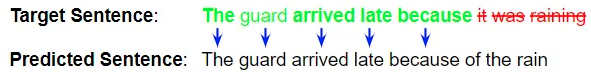
\includegraphics[]{chapters/chapter12/figure/1-gram.png}
    \citebutton{Towards Data Science, Ketan Doshi}{https://towardsdatascience.com/foundations-of-nlp-explained-bleu-score-and-wer-metrics-1a5ba06d812b}
    \label{fig:enter-label}
\end{figure}

\hspace{}

Five out of eight 1-grams are correctly predicted:

\hspace{}

$\rightarrow p_1 = 5/8$

\vfill
    
\end{vbframe}

% ------------------------------------------------------------------------------

\begin{vbframe}{BLEU score (2)}

\begin{figure}
    \centering
    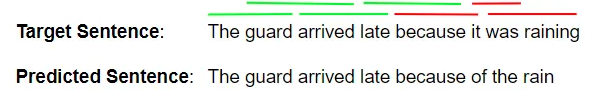
\includegraphics[]{chapters/chapter12/figure/2-gram.png}
    \citebutton{Towards Data Science, Ketan Doshi}{https://towardsdatascience.com/foundations-of-nlp-explained-bleu-score-and-wer-metrics-1a5ba06d812b}
    \label{fig:enter-label}
\end{figure}

\hspace{}

Four out of seven 2-grams are correctly predicted:

\hspace{}

$\rightarrow p_2 = 4/7$

\hspace{}

\textit{You keep doing this procedure until $N$ n-grams and compute a weighted geometric average over the precision scores with weights $w_n$:}

$$exp\left(\sum_{n=1}^{N}w_n\cdot log(p_n)\right)$$
    
\end{vbframe}

% ------------------------------------------------------------------------------

\begin{vbframe}{BLEU Score - Brevity penalty}

\textit{In order to penalize very short predictions (it's more likely for shorter sentences to achieve a good precision score) the BLEU score additionally has a brevity penalty term:}

\hspace{}

$$
  BP=\begin{cases}
    1, & \text{if $c>r$}\\
    e^{(1-r/c)}, & \text{if $c\leq r$}
  \end{cases}
$$

\hspace{}

\begin{itemize}
    \item With $r$ being the \textbf{reference corpus length} and $c$ the \textbf{candidate corpus length}
    \item The final formula is then:

$$BLEU = BP \cdot exp\left(\sum_{n=1}^{N}w_n\cdot log(p_n)\right)$$
\end{itemize}
    
\end{vbframe}


% ------------------------------------------------------------------------------

\begin{vbframe}{ROUGE score}

\vfill

\begin{itemize}
    \item The ROUGE (Recall-Oriented Understudy for Gisting Evaluation) is a metric commonly used for evaluating the quality of machine-generated text, particularly summaries
    \item ROUGE measures the similarity between the generated summary and one or more reference (human-written) summaries
    \item ROUGE includes multiple metrics, such as ROUGE-N (for n-grams), ROUGE-L (for longest common subsequence), and ROUGE-W (for weighted n-grams). Depending on the task, these metrics capture different aspects of summary quality, allowing a more comprehensive evaluation
\end{itemize}

\vfill
    
\end{vbframe}



% ------------------------------------------------------------------------------

\begin{vbframe}{Example: ROUGE-1 precision}

\vfill
\textit{Consider the following source sentence $S$ and candidate summary $C$:}

\hspace{}

\begin{itemize}
    \item \textbf{S:} The cat is on the mat.
    \item \textbf{C:} \textcolor{green}{The cat} and \textcolor{green}{the} dog.
\end{itemize}

\hspace{}

\textit{Using the ROUGE-N precision score with $N = 1$ you get:}

\hspace{}

\begin{itemize}
    \item Three correctly predicted unigrams
    \item Total of number of unigrams in $C$ is 5
\end{itemize}

\hspace{}

$\rightarrow \text{ROUGE-1 precision}=3/5 = 0.6$

\hspace{}

\textit{There are more ROUGE scores as mentioned earlier. You can find more details here:} \citebutton{Medium, Fabio Chiusano}{https://medium.com/nlplanet/two-minutes-nlp-learn-the-rouge-metric-by-examples-f179cc285499}
\vfill
    
\end{vbframe}

% ------------------------------------------------------------------------------
\begin{vbframe}{Metrics without a gold reference}

\vfill

\begin{itemize}
    \item BLEU and ROUGE are both used for tasks that have a gold reference you can compare your prediction to
    \item In open ended text generation you just have a prompt and an output generated by the model
    \item You don't have any gold reference to compare your output to
    \item Therefore you have to get a bit more creative with the choice of evaluation metrics
\end{itemize}



\vfill
    
\end{vbframe}

% ------------------------------------------------------------------------------

\begin{vbframe}{Diversity}
    
\end{vbframe}


% ------------------------------------------------------------------------------

\begin{vbframe}{Coherence}
    
\end{vbframe}

% ------------------------------------------------------------------------------

\begin{vbframe}{MAUVE}
    
\end{vbframe}

% ------------------------------------------------------------------------------

\endlecture
\end{document}